\chapter{Appendix}

\section{Derivation of Equations of motion}
\subsection{Load Dynamics}\label{sec:app.loaddyn}
%PROOF prop.3 Sreenath2013a. Also Sreenath2013b?
%DEFINE e_3 / R / f 

Let \lsymb{$ x_{CM} $}{Position CM of \a{qr}-Load system} denote the position of the center of mass of the combined Quadrotor-Load system, expressed in \IF. Which can be found by
\begin{align}\label{eq:CM}
\begin{split}
m_Q(x_Q-x_{CM})+m_L(x_L-x_{CM})&=0\\
(m_Q+m_L)x_{CM}&=m_Qx_Q+m_Lx_L
\end{split}
\end{align}
Applying Newton's laws of motion to (\ref{eq:CM}) and inserting (\ref{eq:mod.xQ2xL}) gives the 
\begin{align}\label{key}
\begin{split}
(m_Q+m_L)\ddot{x}_{CM}&=fRe_3 - (m_Q+m_L)ge_3\\
%&=fRe_3 - (m_Q+m_L)ge_3\\
%(m_Q+m_L)\ddot{x}_{CM}&=m_Q\ddot{x}_Q + m_L\ddot{x}_L\\
%\\
%m_Q\ddot{x}_Q+m_L\ddot{x}_L&=fRe_3 - (m_Q+m_L)ge_3\\
%m_Q(\ddot{x}_L-L\ddot{q})+m_L\ddot{x}_L&=fRe_3 - (m_Q+m_L)ge_3\\
(m_Q+m_L)(\ddot{x}_L+ge_3)&= fRe_3+m_QL\ddot{q}
\end{split}
\end{align}

%ADD derivation of ddq (TANG2014)
Here comes the derivation of $ \ddot{q} $, obtained by geometric mechanics.

\section{LQR controller}\label{app:lqr}

\subsection{Modeling}
%From Newton's laws follows
%\begin{align}
%x_Q&=fRe_3-m_Qge_3-Tq\\
%x_L&=-m_Lge_3+Tq
%\end{align}
%
%$ x_Q $ and $ x_L $ are related by
%\begin{equation}\label{key}
%x_L = x_Q+Lq
%\end{equation}

%CHECK is dit nodig?
% From Lagrangian equations of motion, 
%
%\begin{equation}\label{eq:app.QRpos}
%\begin{aligned}
%%ADD Not done yet
%\ddot{x}&=\\
%\ddot{y}&=\\
%\ddot{z}&=
%\end{aligned}
%\end{equation}
%
%\begin{equation}\label{eq:app.QRatt}
%\begin{aligned}
%%ADD Not done yet
%\ddot{\phi}&=\\
%\ddot{\theta}&=\\
%\ddot{\psi}&=
%\end{aligned}
%\end{equation}
%
%\begin{equation}\label{eq:app.Latt}
%\begin{aligned}
%%ADD Not done yet
%\ddot{\phi}_L&=\\
%\ddot{\theta}_L&=
%\end{aligned}
%\end{equation}
%The second order system of ODEs can be transformed 
The linearized model is written into a first order ODE of the form
\begin{align}\label{eq:app.ss}
\mathbf{\dot{x} }&=A\mathbf{x}+Bu\\
y&=C\mathbf{x}+Du
\end{align}
with the following state- and input vectors
\begin{equation}\label{key}
\begin{aligned}
%\textbf{x}&=\begin{bmatrix}
%\textbf{q}\\
%\mathbf{\dot{q}}
%\end{bmatrix}\\
%\mathbf{q}&=\begin{bmatrix}
%x&y&z&\phi&\theta&\psi&\phi_L&\theta_L
%\end{bmatrix}^T\\
%\mathbf{\dot{q}}&=\begin{bmatrix}
%\dot{x}&\dot{y}&\dot{z}&\dot{\phi}&\dot{\theta}&\dot{\psi}&\dot{\phi}_L&\dot{\theta}_L
%\end{bmatrix}^T\\
\mathbf{x}&=\begin{bmatrix}
x&y&z&\phi&\theta&\psi&\phi_L&\theta_L&\dot{x}&\dot{y}&\dot{z}&\dot{\phi}&\dot{\theta}&\dot{\psi}&\dot{\phi}_L&\dot{\theta}_L
\end{bmatrix}^T\\
u&=\begin{bmatrix}
f&M_\phi&M_\theta&M_\psi
\end{bmatrix}^T
\end{aligned}
\end{equation}

The model is linearized about the hovering flight mode. All translational and rotational velocities are zero during hover. The positional states and the yaw angle do not affect the dynamics, and are set equal to zero. A thrust input $ u_1=g(mQ+mL) $ is required to maintain hover, and all other control inputs are set equal to zero. 
The states and inputs in the equations of motion are substituted by an initial condition and a perturbation
\begin{equation}\label{key}
\mathbf{\dot{x}}\rightarrow\mathbf{\dot{x}}_0+\delta\mathbf{\dot{x}}, \quad \mathbf{{x}}\rightarrow\mathbf{{x}}_0+\delta\mathbf{{x}}, \quad u\rightarrow u_0+\delta u
\end{equation}
\begin{equation}\label{key}
\begin{aligned}
\mathbf{x}(0) &= \mathbf{0}\\
u(0)&=\begin{bmatrix}
g(m_Q+m_L) &0 &0& 0
\end{bmatrix}^T
\end{aligned}
\end{equation}
The linearized equations of motion are rearranged into Equation \ref{eq:app.2ode} and substituted in Equation \ref{eq:app.ss}.
\begin{equation}\label{eq:app.2ode}
\begin{bmatrix}
content...
\end{bmatrix}
\begin{bmatrix}
		\delta \ddot{x} \\\delta\ddot{y}\\\delta\ddot{z}\\\delta\ddot{\phi}\\\delta\ddot{\theta}\\\delta\ddot{\psi}\\\delta\ddot{\phi}_L\\\delta\ddot{\theta}_L 
		\end{bmatrix}+
\begin{bmatrix}
content...
\end{bmatrix}
\begin{bmatrix}
		\delta {x} \\\delta{y}\\\delta{z}\\\delta{\phi}\\\delta{\theta}\\\delta{\psi}\\\delta{\phi}_L\\\delta{\theta}_L 
\end{bmatrix}
=
\begin{bmatrix}
content...
\end{bmatrix}
\begin{bmatrix}
\delta u_1\\\delta u_2\\\delta u_3\\\delta u_4
\end{bmatrix}
\end{equation}

%ADD LQRA
\begin{lstlisting}
LQRA =

\end{lstlisting}
%ADD LQRB
\begin{lstlisting}
LQRB =

\end{lstlisting}
The tuning parameters of the \a{lqr} controller a chosen as follows
%TEST different values LQR
\begin{equation}\label{key}
\begin{aligned}
Q &= diag\begin{pmatrix}
10 &10 &100,& 1& 1& 1, &1& 1,& 1& 1 &1,& 1& 1& 1,& 1& 1
\end{pmatrix}\\
R &= diag\begin{pmatrix}
0.044, &1.56,& 1.56, &1.56
\end{pmatrix}
\end{aligned}
\end{equation}
\texttt{Matlab} command \texttt{lqr(LQRA,LQRB,Q,R)} generates the following gain matrix $ K $
%ADD K
\begin{lstlisting}
K =

\end{lstlisting}




%CHECK useful? Praveen EOM
%	    \begin{equation}
%	    ax = 
%	    \begin{bmatrix}
%	    f(ms_{\phi_q}s_{\psi_q}+ m_Ls_{\phi_q}s_{\psi_q} + mc_{\phi_q}c_{\psi_q}s_{\theta_q} + m_Lc_{\phi_q}c_{\psi_q}s_{\theta_q}- m_Lc_{\phi_q}c_{\psi_q}c_{\theta}^2s_{\theta_q} + m_Lc_{\phi}^2c_{\phi_q}c_{\psi_q}c_{\theta}^2s_{\theta_q} - m_Lc_{\theta}^2s_{\phi_q}s_{\psi_q}+ m_Lc_{\phi}^2c_{\theta}^2s_{\phi_q}s_{\psi_q}  + m_Lc_{\psi_q}c_{\theta}s_{\phi}s_{\phi_q}s_{\theta} + m_Lc_{\phi}c_{\phi_q}c_{\theta_q}c_{\theta}^2s_{\phi} - m_Lc_{\phi_q}c_{\theta}s_{\phi}s_{\psi_q}s_{\theta_q}s_{\theta})
%	    
%	    
%	    (   + Lmm_Lv_\theta^2c_{\theta}s_{\phi} + Lmm_Lv_\phi^2c_{\theta}^3s_{\phi} )/(m(m + m_L))\\
%	    \\
%	    (Lmm_Lv_\theta^2s_{\theta} - fm_Lc_{\psi_q}c_{\theta}^2s_{\phi_q} - fmc_{\psi_q}s_{\phi_q} + fmc_{\phi_q}s_{\psi_q}s_{\theta_q} + fm_Lc_{\phi_q}c_{\theta}^2s_{\psi_q}s_{\theta_q} + Lmm_Lv_\phi^2c_{\theta}^2s_{\theta} + fm_Lc_{\phi}c_{\phi_q}c_{\theta_q}c_{\theta}s_{\theta} - fm_Lc_{\theta}s_{\phi}s_{\phi_q}s_{\psi_q}s_{\theta} - fm_Lc_{\phi_q}c_{\psi_q}c_{\theta}s_{\phi}s_{\theta_q}s_{\theta})/(m(m + m_L))\\
%	    \\
%	    -(gm^2 + gmm_L - fmc_{\phi_q}c_{\theta_q} - fm_Lc_{\phi_q}c_{\theta_q} + Lmm_Lv_\theta^2c_{\phi}c_{\theta} + fm_Lc_{\phi}^2c_{\phi_q}c_{\theta_q}c_{\theta}^2 + Lmm_Lv_\phi^2c_{\phi}c_{\theta}^3 + fm_Lc_{\phi}c_{\psi_q}c_{\theta}s_{\phi_q}s_{\theta} - fm_Lc_{\phi}c_{\theta}^2s_{\phi}s_{\phi_q}s_{\psi_q} - fm_Lc_{\phi}c_{\phi_q}c_{\theta}s_{\psi_q}s_{\theta_q}s_{\theta} - fm_Lc_{\phi}c_{\phi_q}c_{\psi_q}c_{\theta}^2s_{\phi}s_{\theta_q})/(m(m + m_L))\\
%	    \\
%	    (- Lmc_{\theta}s_{\theta}v_\phi^2 + fc_{\psi_q}c_{\theta}s_{\phi_q} - fc_{\phi}c_{\phi_q}c_{\theta_q}s_{\theta} - fc_{\phi_q}c_{\theta}s_{\psi_q}s_{\theta_q} + fs_{\phi}s_{\phi_q}s_{\psi_q}s_{\theta} + fc_{\phi_q}c_{\psi_q}s_{\phi}s_{\theta_q}s_{\theta})/(Lm)\\
%	    \\
%	    -(fc_{\phi_q}c_{\theta_q}s_{\phi} + fc_{\phi}s_{\phi_q}s_{\psi_q} - 2Lmv_\phi v_{\theta}s_{\theta} + fc_{\phi}c_{\phi_q}c_{\psi_q}s_{\theta_q})/(Lmc_{\theta})
%	    \end{bmatrix}
%	    \end{equation}	    
%	    
%	    ***************************************\\	

\section{Classical Modeling}\label{sec:mod.clas}
This section describes the derivation of the model by using classical modeling techniques.

When assuming small angle maneuvers, \textit{Euler-angles} can be used to locally parameterize the orientation of the body-fixed reference coordinate frame with respect to the inertial reference coordinate frame. Simple linear controllers are often based on a linearized dynamical model, applying this small angles assumption. 

\begin{figure}[h!]
	\centering
	\makebox[.65\textwidth][c]{\subfloat[][Quadrotor model representation \label{fig:app.model}]{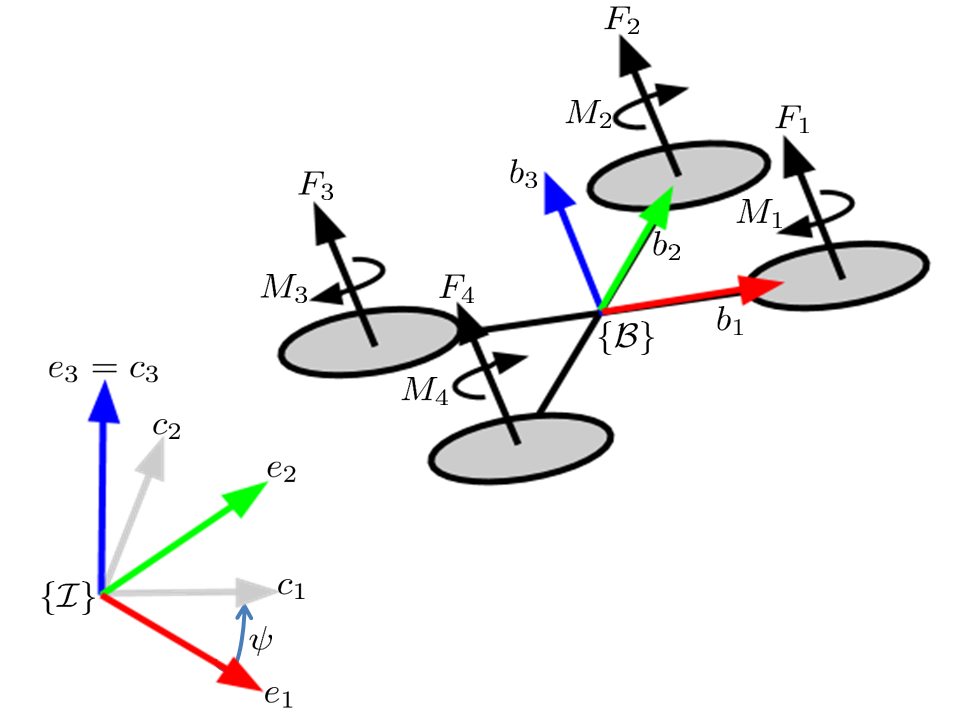
\includegraphics[width=.5\textwidth]{./StyleStuff/qrmodel.png}}}
	\makebox[.34\textwidth][c]{\subfloat[][Load angles  \label{fig:app.angles}]{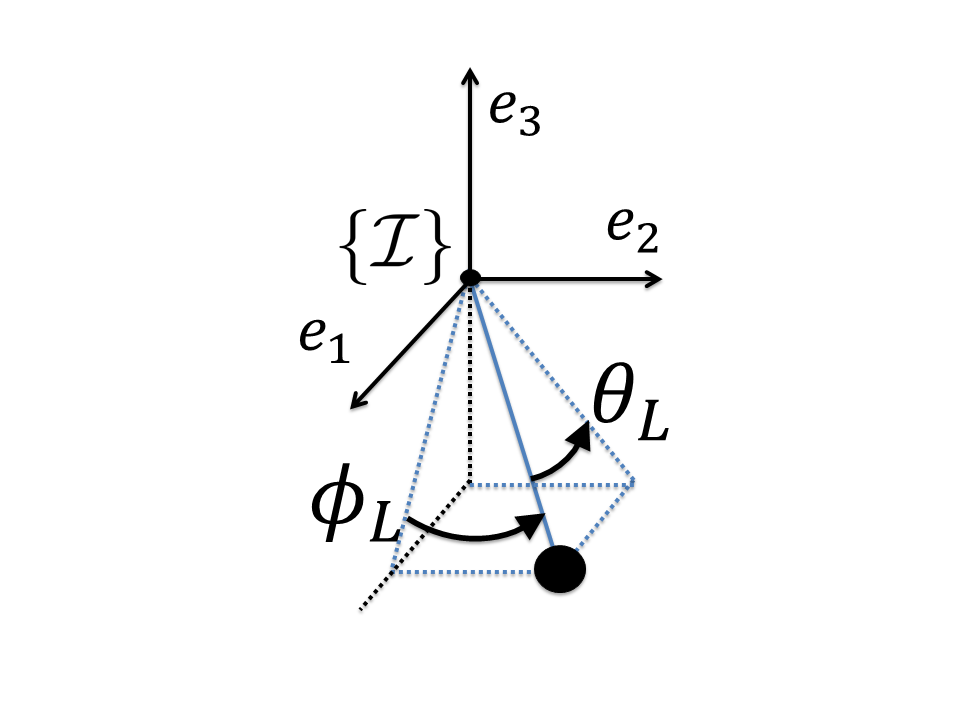
\includegraphics[width=.5\textwidth]{./StyleStuff/angles.png}}}
	\caption{Model representation\label{fig:}}
\end{figure}		

The following equations of motion follow from Newton's law.
\begin{equation}\label{eq:newton}
\begin{aligned}
\dot{x}_Q &= v_Q\\
m_Q\dot{v}_Q &=fRe_3-m_Qge_3-Tq\\
\dot{x}_L &= v_L\\
m_L\dot{v}_L &=-m_Lge_3+Tq
\end{aligned}
\end{equation}
where $ x_Q = x_L-Lq $. $ T $ is the cable tension, defined by $ T=|f| q $, where $ |f| = m_L\dot{v}_L $ is the magnitude of the force.
%which gives the following equation, derived in Section \ref{sec.app:loaddyn},
%\begin{equation}\label{key}
%%CHECK whether equation is correct
%(m_Q+m_L)(\dot{v}_L+ge_3)=fRe_3-m_QL\ddot{q}
%\end{equation}

Because Euler-Angles are used, a function is required that maps a vector of the Z-X-Y Euler angles to its rotation matrix $ R\in SO(3) $, which is denoted as \cite{Mahony2012}
\begin{equation}\label{key}
R_{ZXY}({\phi},{\theta},{\psi})=\begin{bmatrix}
c_{\psi}c_{\theta}-s_{\phi}s_{\psi}s_{\theta}&-c_{\phi}s_{\psi}&c_{\psi}s_{\theta}+c_{\theta}s_{\phi}s_{\psi}\\
c_{\theta}s_{\psi}+c_{\psi}s_{\phi}s_{\theta}&c_{\phi}c_{\psi}&s_{\psi}s_{\theta}-c_{\psi}c_{\theta}s_{\phi}\\
-c_{\phi}s_{\theta}&s_{\phi}&c_{\phi}c_{\theta}
\end{bmatrix}
\end{equation}
The Z-X-Y Euler angles rotate \BF, as can be seen in Figure \ref{fig:app.model}. The first rotation by yaw angle $ \psi $ is around the z-axis of \IF. Next is the rotation by roll angle $ \phi $, and the last rotation is by pitch angle $ \theta $.
%\begin{figure}[h!]
%	\centering
%	\makebox[\textwidth][c]{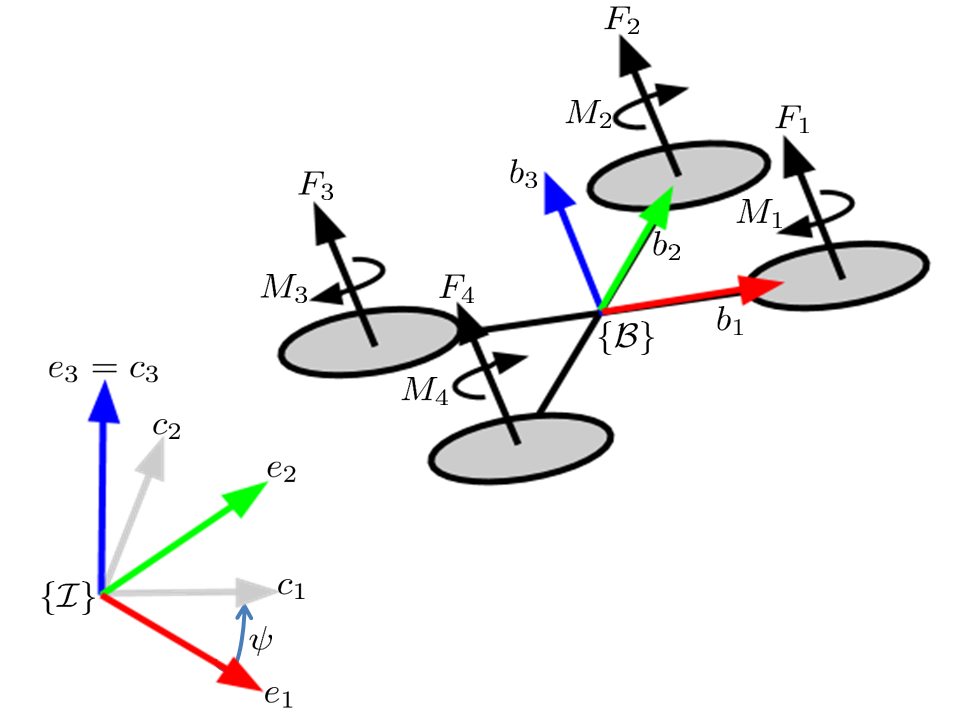
\includegraphics[width=.45\textwidth]{./StyleStuff/qrmodel.png}}
%	\caption{Quadrotor-Load model representation\label{fig:mod.modelQRtrad}}
%\end{figure}

The unit vector $ q $ from the \a{qr} to the load is represented in \BF. Define $ \phi_L $ as the rotation of the load around the z-axis, measured from $ \vec{b}_1 $, and $ \theta_L $ is the angle between the cable and the z-axis of \BF, see Figure \ref{fig:app.angles}.
The Cartesian coordinates can be retrieved through
\begin{equation}\label{eq:app.xL2xQ}
x_L = x_Q+qL
\end{equation}
where
\begin{equation}\label{eq:app.q}
q=
\begin{bmatrix}
s_{\theta_L}c_{\phi_L}\\
s_{\theta_L}s_{\phi_L}\\
-c_{\theta_L}
\end{bmatrix}
\end{equation}
%\begin{figure}[h!]
%	\centering
%	\makebox[\textwidth][c]{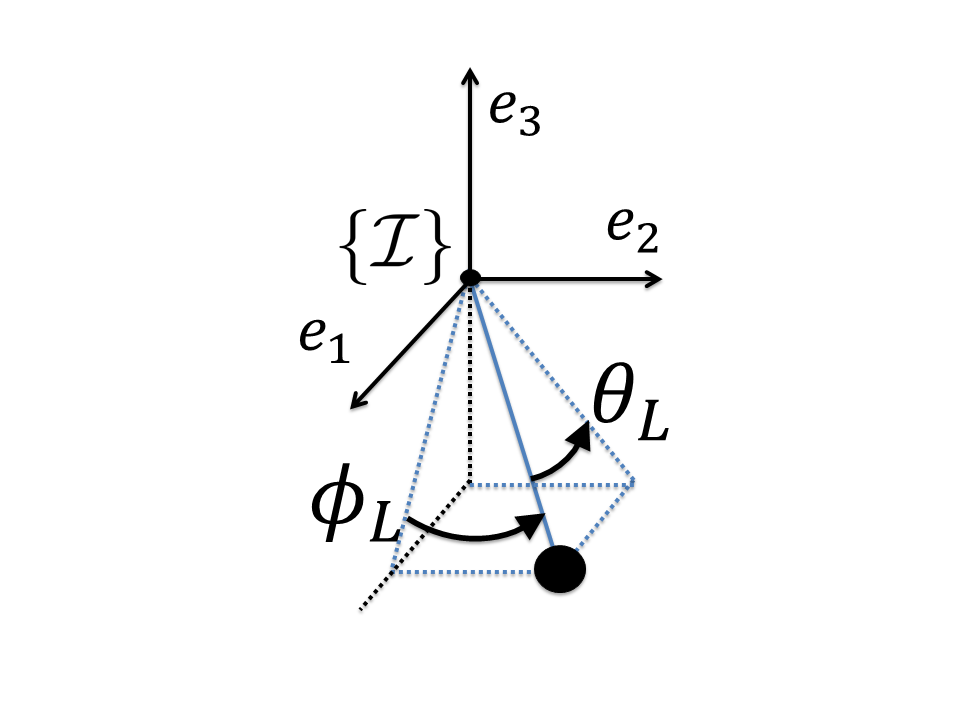
\includegraphics[width=.45\textwidth]{./StyleStuff/angles.png}}
%	\caption{Load angles \label{fig:app.angles}}
%\end{figure}	

%\begin{figure}[h!]
%	\centering
%	\makebox[\textwidth][c]{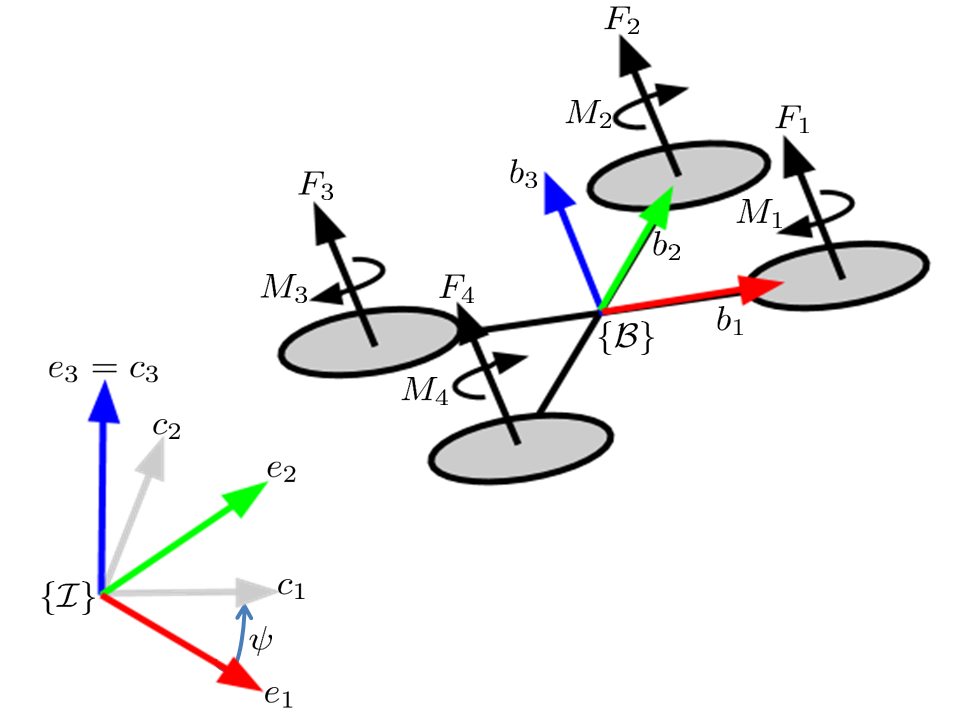
\includegraphics[width=.5\paperwidth]{./StyleStuff/qrmodel.png}}
%	\caption{Quadrotor model representation\label{fig:mod.model}}
%\end{figure}	



%\begin{equation}\label{eq:q}
%		q=-R_{\psi_L}R_{\theta_L}e_3=\begin{bmatrix}
%		s_{\theta_L}c_{\psi_L}\\s_{\theta_L}s_{\psi_L}\\-c_{\theta_L}
%		\end{bmatrix}
%\begin{align}
%q=\begin{bmatrix}
%s_{\theta_L}c_{\phi_L}\\
%s_{\theta_L}s_{\phi_L}\\
%c_{\theta_L}
%\end{bmatrix}
%\dot{q}&=\begin{bmatrix}
%s_{\theta_L}c_{\psi_L}\\
%s_{\theta_L}s_{\psi_L}\\
%c_{\theta_L}
%\end{bmatrix}\\
%\end{align}
%\end{equation}  
Differentiating Equation \ref{eq:app.xL2xQ} and \ref{eq:app.q} gives
\begin{equation}\label{key}
\begin{aligned}
\ddot{x}_L&=\ddot{x}_Q+\ddot{q}L\\
\ddot{q}&=\begin{bmatrix}
\ddot{\theta}_Lc_{\theta_L}c_{\phi_L}-\ddot{\phi}_Ls_{\theta_L}s_{\phi_L}-\dot{\phi}_L^2s_{\theta_L}c_{\phi_L}-\dot{\theta}_L^2s_{\theta_L}c_{\phi_L}-2\dot{\theta}_L\dot{\phi}_Lc_{\theta_L}s_{\phi_L}\\
\ddot{\theta}_Lc_{\theta_L}s_{\phi_L}+\ddot{\phi}_Ls_{\theta_L}c_{\phi_L}-\dot{\phi}_L^2s_{\theta_L}s_{\phi_L}-\dot{\theta}_L^2s_{\theta_L}s_{\phi_L}+2\dot{\theta}_L\dot{\phi}_Lc_{\theta_L}c_{\phi_L}\\
\ddot{\theta}_Ls_{\theta_L}+\dot{\theta}_L^2 c_{\theta_L}\\
\end{bmatrix}
\end{aligned}
\end{equation}

\begin{equation}\label{key}
\begin{aligned}
\ddot{x}_Q&=\frac{1}{m_Q}(f(c_{\psi}s_{\theta}+c_{\theta}s_{\phi}s_{\psi})-Ts_{\theta_L}c_{\psi_L})\\
\ddot{y}_Q&=\frac{1}{m_Q}(f(s_{\psi}s_{\theta}-c_{\psi}c_{\theta}s_{\phi})-Ts_{\theta_L}s_{\psi_L})\\
\ddot{z}_Q&=\frac{1}{m_Q}(f(c_{\phi}c_{\theta})-Tc_{\theta_L})-g\\
\end{aligned}
\end{equation}

%\begin{align}\label{key}
%%CHECK wat is hier de bedoeling van? Checken in Garcia of literatuur?
%\ddot{\psi}&=\tilde{\tau}_{\psi}\\
%\ddot{\theta}&=\tilde{\tau}_{\theta}\\
%\ddot{\phi} &=\tilde{\tau}_{\phi}
%\end{align}

\section{Derivation Error dynamics}\label{sec:app.error}
\subsection{Quadrotor Attitude}
From the angular velocity tracking error $ e_\Omega $ follows
\begin{equation}\label{eq:app.eOmega}
\begin{aligned}
e_\Omega&=\Omega-R^TR_d\Omega_d,\\
\hat{e}_\Omega&=\hat{\Omega}-R^TR_d\hat{\Omega}_dR_d^TR
\end{aligned}
\end{equation}

The attitude tracking and its time derivative is given by
\begin{equation}\label{key}
\begin{aligned}
e_R&=\frac{1}{2}(R_d^TR-R^TR_d)^\vee,\\
\dot{e}_R&=\frac{1}{2}(\dot{R}_d^TR+R_d^T\dot{R}-\dot{R}^TR_d-R^T\dot{R}_d)^\vee\\
&=\frac{1}{2}((R_d\hat{\Omega}_d)^TR+R_d^T(R\hat{\Omega})-(R\hat{\Omega})^TR_d-R^T(R_d\hat{\Omega}_d))^\vee\\
&=\frac{1}{2}(-\hat{\Omega}_dR_d^TR+R_d^TR\hat{\Omega}+\hat{\Omega}R^TR_d-R^TR_d\hat{\Omega}_d)^\vee\\
&=\frac{1}{2}(R_d^TR(\hat{\Omega}-R^TR_d\hat{\Omega}_dR_d^TR)+(\hat{\Omega}-R^TR_d\hat{\Omega}_dR_d^TR)R^TR_d)^\vee
%&=\frac{1}{2}(R_d^TR\hat{e}_\Omega+\hat{e}_\Omega R^TR_d)^\vee\\
%&=\frac{1}{2}(tr[R^TR_d]I-R^TR_d)e_\Omega \equiv C(R_d^TR)e_\Omega
\end{aligned}
\end{equation}

\begin{equation}\label{key}
\begin{aligned}
\dot{e}_\Omega&=\dot{\Omega}-\dot{R}^TR_d\Omega_d-R^T\dot{R}_d\Omega_d-R^TR_d\dot{\Omega}_d\\
&=\dot{\Omega}-(R\hat{\Omega})^TR_d\Omega_d-R^T({R}_d\hat{\Omega}_d)\Omega_d-R^TR_d\dot{\Omega}_d\\
&=\dot{\Omega}+\hat{\Omega}R^TR_d\Omega_d-R^T({R}_d\hat{\Omega}_d)\Omega_d-R^TR_d\dot{\Omega}_d\\
&=J^{-1}(-\Omega\times J\Omega + M)+\hat{\Omega}R^TR_d\Omega_d-R^TR_d\dot{\Omega}_d
\end{aligned}
\end{equation}
where $\hat{\Omega}_d\Omega_d=\Omega_d \times \Omega_d=0  $.

\section{Figures}
%CHECK nodig?
\begin{figure}[h!]
	\centering
	\makebox[\textwidth][c]{\includegraphics[width=.45\textwidth]{./StyleStuff/dcsc.png}}
	\caption{Simulink Command Filter\label{fig:app.CF}}
\end{figure}		

%\section{\texttt{MATLAB} code}
%\subsection{A \matlab Listing}
%
%\lstset{language=matlab}
%\lstinputlisting{test.m}

%    \subsection{An appendix subsection with C++ Listing}
%
%    \lstset{language=C++}
%    \lstinputlisting{test.c}    

%    \chapter{Appendix: Figures}
%
%    \section{Test section (again?)}
%
%    Ok, all is well.